% Options for packages loaded elsewhere
\PassOptionsToPackage{unicode}{hyperref}
\PassOptionsToPackage{hyphens}{url}
%
\documentclass[
]{article}
\usepackage{amsmath,amssymb}
\usepackage{lmodern}
\usepackage{iftex}
\ifPDFTeX
  \usepackage[T1]{fontenc}
  \usepackage[utf8]{inputenc}
  \usepackage{textcomp} % provide euro and other symbols
\else % if luatex or xetex
  \usepackage{unicode-math}
  \defaultfontfeatures{Scale=MatchLowercase}
  \defaultfontfeatures[\rmfamily]{Ligatures=TeX,Scale=1}
\fi
% Use upquote if available, for straight quotes in verbatim environments
\IfFileExists{upquote.sty}{\usepackage{upquote}}{}
\IfFileExists{microtype.sty}{% use microtype if available
  \usepackage[]{microtype}
  \UseMicrotypeSet[protrusion]{basicmath} % disable protrusion for tt fonts
}{}
\makeatletter
\@ifundefined{KOMAClassName}{% if non-KOMA class
  \IfFileExists{parskip.sty}{%
    \usepackage{parskip}
  }{% else
    \setlength{\parindent}{0pt}
    \setlength{\parskip}{6pt plus 2pt minus 1pt}}
}{% if KOMA class
  \KOMAoptions{parskip=half}}
\makeatother
\usepackage{xcolor}
\usepackage{longtable,booktabs,array}
\usepackage{calc} % for calculating minipage widths
% Correct order of tables after \paragraph or \subparagraph
\usepackage{etoolbox}
\makeatletter
\patchcmd\longtable{\par}{\if@noskipsec\mbox{}\fi\par}{}{}
\makeatother
% Allow footnotes in longtable head/foot
\IfFileExists{footnotehyper.sty}{\usepackage{footnotehyper}}{\usepackage{footnote}}
\makesavenoteenv{longtable}
\usepackage{graphicx}
\makeatletter
\def\maxwidth{\ifdim\Gin@nat@width>\linewidth\linewidth\else\Gin@nat@width\fi}
\def\maxheight{\ifdim\Gin@nat@height>\textheight\textheight\else\Gin@nat@height\fi}
\makeatother
% Scale images if necessary, so that they will not overflow the page
% margins by default, and it is still possible to overwrite the defaults
% using explicit options in \includegraphics[width, height, ...]{}
\setkeys{Gin}{width=\maxwidth,height=\maxheight,keepaspectratio}
% Set default figure placement to htbp
\makeatletter
\def\fps@figure{htbp}
\makeatother
\usepackage[normalem]{ulem}
\setlength{\emergencystretch}{3em} % prevent overfull lines
\providecommand{\tightlist}{%
  \setlength{\itemsep}{0pt}\setlength{\parskip}{0pt}}
\setcounter{secnumdepth}{-\maxdimen} % remove section numbering
\ifLuaTeX
  \usepackage{selnolig}  % disable illegal ligatures
\fi
\IfFileExists{bookmark.sty}{\usepackage{bookmark}}{\usepackage{hyperref}}
\IfFileExists{xurl.sty}{\usepackage{xurl}}{} % add URL line breaks if available
\urlstyle{same} % disable monospaced font for URLs
\hypersetup{
  hidelinks,
  pdfcreator={LaTeX via pandoc}}

\author{}
\date{}

\begin{document}

\begin{quote}

\includegraphics[width=1.36597in,height=0.98264in]{vertopal_24f0430788374a81b8d4c0bb6e5080ec/media/image1.jpeg}IC-201P

\textbf{PROJECT REPORT- GROUP 07}

\uline{WASTE COLLECTION MANAGEMENT SYSTEM FOR}

\uline{IIT MANDI}
\end{quote}


\includegraphics[width=6.5in,height=\textheight]{vertopal_24f0430788374a81b8d4c0bb6e5080ec/media/image2.png}

\hypertarget{faculty-mentors}{%
\subsubsection{\texorpdfstring{ \textbf{FACULTY
MENTORS:}}{ FACULTY MENTORS:}}\label{faculty-mentors}}

\begin{itemize}
\item
  \textbf{Dr. Sarthak Nag}
\item
  \textbf{Dr. Pramod Kumar}
\end{itemize}

\begin{longtable}[]{@{}
  >{\raggedright\arraybackslash}p{(\columnwidth - 2\tabcolsep) * \real{0.4955}}
  >{\raggedright\arraybackslash}p{(\columnwidth - 2\tabcolsep) * \real{0.5045}}@{}}
\toprule()
\begin{minipage}[b]{\linewidth}\raggedright
\begin{quote}
\textbf{Name}
\end{quote}
\end{minipage} & \begin{minipage}[b]{\linewidth}\raggedright
\begin{quote}
\textbf{Roll No.}
\end{quote}
\end{minipage} \\
\midrule()
\endhead
\begin{minipage}[t]{\linewidth}\raggedright
\begin{quote}
Arendra Kumar
\end{quote}
\end{minipage} & \begin{minipage}[t]{\linewidth}\raggedright
\begin{quote}
B23394
\end{quote}
\end{minipage} \\
\begin{minipage}[t]{\linewidth}\raggedright
\begin{quote}
Dipanshu
\end{quote}
\end{minipage} & \begin{minipage}[t]{\linewidth}\raggedright
\begin{quote}
B23126
\end{quote}
\end{minipage} \\
\begin{minipage}[t]{\linewidth}\raggedright
\begin{quote}
Utkarsh
\end{quote}
\end{minipage} & \begin{minipage}[t]{\linewidth}\raggedright
\begin{quote}
B23056
\end{quote}
\end{minipage} \\
\begin{minipage}[t]{\linewidth}\raggedright
\begin{quote}
Anuj Pal
\end{quote}
\end{minipage} & \begin{minipage}[t]{\linewidth}\raggedright
\begin{quote}
B23339
\end{quote}
\end{minipage} \\
\begin{minipage}[t]{\linewidth}\raggedright
\begin{quote}
Keshav Kumar
\end{quote}
\end{minipage} & \begin{minipage}[t]{\linewidth}\raggedright
\begin{quote}
B23076
\end{quote}
\end{minipage} \\
\begin{minipage}[t]{\linewidth}\raggedright
\begin{quote}
Vulli Navadheer Kumar
\end{quote}
\end{minipage} & \begin{minipage}[t]{\linewidth}\raggedright
\begin{quote}
B23361
\end{quote}
\end{minipage} \\
Yash Taneja (TA) & D23116 \\
Dipanshu Thakur

(Student Buddy) & B22037 \\
\bottomrule()
\end{longtable}

\hypertarget{introduction-to-the-problem-statement-and-its-need}{%
\section{\texorpdfstring{ INTRODUCTION TO THE PROBLEM STATEMENT AND ITS
NEED}{ INTRODUCTION TO THE PROBLEM STATEMENT AND ITS NEED}}\label{introduction-to-the-problem-statement-and-its-need}}

\hypertarget{section}{%
\section{}\label{section}}

\begin{quote}
IIT Mandi, located in the picturesque hills of Himachal Pradesh, is
committed to maintaining an eco-friendly and sustainable campus. As the
number of students, faculty, and staff continues to grow, so does the
volume of waste generated across various campus facilities. This
increasing waste presents a challenge that needs to be addressed to
preserve the campus\textquotesingle s natural beauty and minimize
environmental impact.

The waste generated at IIT Mandi comes from diverse sources, including
student hostels, mess facilities, cafes, laboratories, and
administrative buildings. This waste includes biodegradable food scraps,
non-biodegradable plastics, and electronic waste, each requiring
different management approaches. The varied nature of this waste
underscores the need for a robust waste collection and management
system.

Segregating waste into biodegradable, non-biodegradable, and recyclable
categories at the point of collection is crucial for effective
management of the waste. By systematically recycling plastics and
organic waste, we can transform them into valuable resources like
compost and reusable products.

A structured waste management system will improve campus cleanliness,
reduce pest infestations, and promote a healthier environment for
everyone. Engaging students, faculty, and staff in waste segregation and
disposal encourages a culture of environmental responsibility and
sustainability.
\end{quote}

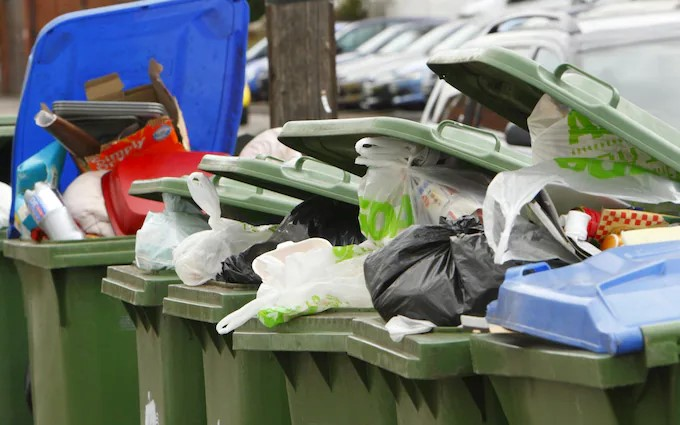
\includegraphics[width=2.66667in,height=2.41181in]{vertopal_24f0430788374a81b8d4c0bb6e5080ec/media/image3.jpeg}
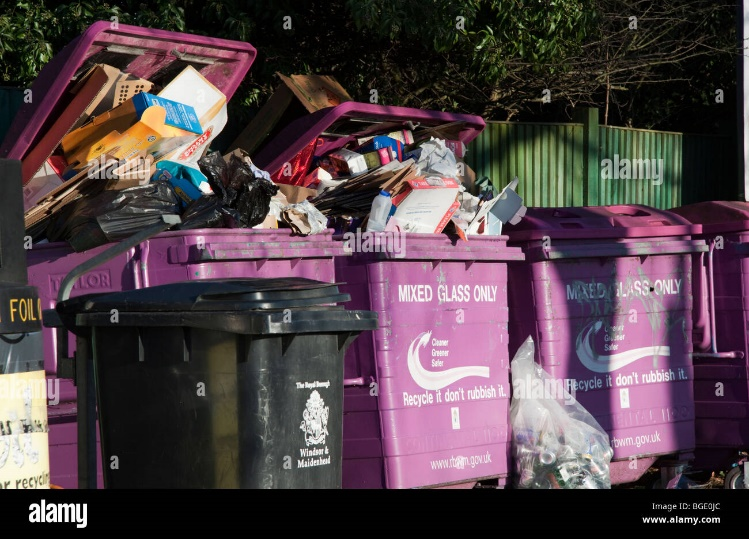
\includegraphics[width=2.64167in,height=2.41181in]{vertopal_24f0430788374a81b8d4c0bb6e5080ec/media/image4.jpeg}

\hypertarget{possible-solutions}{%
\section{POSSIBLE SOLUTIONS}\label{possible-solutions}}

\hypertarget{dustbin-modification-approaches}{%
\subsubsection{\texorpdfstring{\emph{\textbf{1}. \textbf{Dustbin
Modification
Approaches}}}{1. Dustbin Modification Approaches}}\label{dustbin-modification-approaches}}

\begin{itemize}
\item
  \textbf{Compressed Air-Powered Trash Collection}: This concept
  involves designing bins with compressible air bags that compress waste
  to reduce its volume. By decreasing the space occupied by waste, it
  helps in addressing storage issues and allows for less frequent waste
  collection.
\item
  \textbf{Solar-powered Trash Compactor Bin}: These bins use solar power
  to compact the waste inside them, reducing the volume of trash
  collected. By increasing the bin's capacity, it lowers the frequency
  of waste collection while being energy-efficient and sustainable.
\item
  \textbf{Smart Waste Segregation Bins with Arduino}: Utilizing Arduino
  microcontrollers and sensors, this system automatically detects the
  type of waste (organic, recyclable, non-recyclable) and opens the
  appropriate compartment for segregation, improving efficiency and
  accuracy in waste management.
\end{itemize}

\hypertarget{app-integration-approaches}{%
\subsubsection{\texorpdfstring{\emph{\textbf{2. App Integration
Approaches}}}{2. App Integration Approaches}}\label{app-integration-approaches}}

\begin{itemize}
\item
  \textbf{App for Waste Collection Management}: This is a versatile app
  that can manage various waste-related tasks, such as tracking waste
  collection, monitoring bin status, and even providing users with
  insights on how to reduce waste generation. It can be integrated with
  sensors in bins to offer real-time updates
\item
  \textbf{Location-based Garbage Management System}: This idea involves
  capturing a photo of filled trash cans along with their location and
  uploading them to an app. The system allows users to notify
  authorities when bins need to be emptied, making the process more
  efficient
\item
  \textbf{Smart Bin with Sensors and QR code}: These bins have built-in
  sensors that detect when they are full and send an alert to waste
  management personnel, ensuring timely waste collection without manual
  checks.
\item
  \textbf{Upcycling and Reverse Vending App}: This app encourages users
  to recycle and upcycle waste by offering rewards for recycling
  containers via reverse vending machines. It also allows users to
  upload creative ideas for reusing waste.
\end{itemize}

\hypertarget{recycling-and-reusing-approaches}{%
\subsubsection{\texorpdfstring{\emph{\textbf{3. Recycling and Reusing
Approaches}}}{3. Recycling and Reusing Approaches}}\label{recycling-and-reusing-approaches}}

\begin{itemize}
\item
  \textbf{Plastic Waste to 3D Printer Filament}: This approach focuses
  on recycling plastic waste by converting it into filaments used for 3D
  printing. It promotes a circular economy by repurposing waste
  materials for the creation of new objects and prototypes.
\item
  \textbf{Waste to Brick}: The idea involves using waste materials to
  form bricks, which can be used in construction. This promotes
  sustainable building practices and reduces the environmental impact of
  traditional brick manufacturing.
\item
  \textbf{Integrated Approach for Organic and Plastic Waste}: This
  involves combining different techniques, such as using plastic bottles
  to create greenhouses while employing anaerobic digestion to convert
  organic waste into useful by-products like biogas and compost.
\end{itemize}

\hypertarget{advanced-waste-processing-approaches}{%
\subsubsection{\texorpdfstring{4. \emph{\textbf{Advanced Waste
Processing
Approaches}}}{4. Advanced Waste Processing Approaches}}\label{advanced-waste-processing-approaches}}

\begin{itemize}
\item
  \textbf{Automated Litter Detection Drone}: This concept utilizes
  drones equipped with cameras and AI to detect litter across campus
  grounds. The drone can either notify personnel of the
  litter\textquotesingle s location or autonomously collect and dispose
  of it.
\item
  \textbf{AI-Assisted Recycling}: AI technology is used to sort waste in
  recycling centers. Using image processing, the AI system can identify
  different types of waste and separate them accordingly. This process
  can be enhanced by using vacuum systems for picking up waste.
\end{itemize}

\hypertarget{sustainability-oriented-approaches}{%
\subsubsection{\texorpdfstring{5\emph{. \textbf{Sustainability-Oriented
Approaches}}}{5. Sustainability-Oriented Approaches}}\label{sustainability-oriented-approaches}}

\begin{itemize}
\item
  \textbf{Compost Pit System with Automated Aeration}: This system
  accelerates the composting process by automatically regulating airflow
  in compost pits. By doing so, it improves the efficiency of organic
  waste decomposition and supports sustainable waste management.
\item
  \textbf{Converting Organic Waste into Biogas}: Organic waste is
  decomposed in controlled conditions to produce biogas, which can be
  used as an alternative to LPG. This approach not only reduces waste
  but also provides a renewable energy source.
\end{itemize}

\hypertarget{our-solution}{%
\section{OUR SOLUTION}\label{our-solution}}

\begin{quote}
The proposed solution is a \textbf{Smart Waste Segregation Bin} designed
to enhance waste collection efficiency at IIT Mandi. The bin is equipped
with sensors to automatically detect the type of waste---biodegradable,
non-biodegradable, or other--- and segregate it accordingly. An
accompanying mobile app offers users multiple features for interaction
and engagement, supporting the institution's goal of promoting
sustainable waste management.
\end{quote}

\hypertarget{smart-bin-features}{%
\paragraph{\texorpdfstring{\textbf{Smart Bin
Features:}}{Smart Bin Features:}}\label{smart-bin-features}}

\begin{enumerate}
\def\labelenumi{\arabic{enumi}.}
\item
  \textbf{Automatic Waste Segregation:}

  \begin{itemize}
  \item
    The bin features \textbf{optical module and sensors} installed
    centrally to detect the type of waste deposited.
  \item
    Based on the detected waste type, the corresponding compartment's
    \textbf{automatic lid} opens to allow correct disposal.
  \item
    The waste is segregated into \textbf{three categories}:
    biodegradable, non-biodegradable, and others.
  \end{itemize}
\item
  \textbf{Design and Durability:}

  \begin{itemize}
  \item
    Constructed using durable materials such as stainless steel or
    weather-resistant plastic, the bin is suitable for both indoor and
    outdoor environments.
  \item
    Optional \textbf{solar panels} provide a sustainable power source
    for operating the sensors and motorized lids, reducing energy
    consumption.
  \end{itemize}
\item
  \textbf{App Integration:}

  \begin{itemize}
  \item
    The bin is fitted with \textbf{App-Integration} to measure its waste
    capacity in real time, which is displayed on the app.
  \item
    Notifications are automatically triggered to the waste management
    team when a bin is full, ensuring timely disposal and reducing
    manual checking
  \item
  \end{itemize}
\end{enumerate}

\hypertarget{mobile-app-integration}{%
\paragraph{\texorpdfstring{\textbf{Mobile App
Integration:}}{Mobile App Integration:}}\label{mobile-app-integration}}

The smart bin is paired with a mobile application that offers modern
features, making waste management at IIT Mandi more efficient and
interactive. The app encourages community involvement through:

\begin{itemize}
\item
  \textbf{Fullness Indicator}: Users and waste management staff are
  notified when the bin is nearing full capacity, improving collection
  efficiency.
\item
  \textbf{Real-Time Monitoring}: The app allows for monitoring the fill
  level of bins across the campus, with alerts for when waste collection
  is required.
\item
  \textbf{Rewards System}: Users can submit waste recycling ideas and
  earn rewards or points through the app. This feature encourages
  innovation and active participation in reducing campus waste.
\item
  \textbf{Waste Analytics}: The app logs data on the amount of waste
  generated, providing valuable insights into waste management practices
  at IIT Mandi. This data will help optimize collection routes and waste
  reduction strategies.
\item
  \textbf{QR Code Access}: Each bin is equipped with a QR code for users
  to scan. This provides real-time information on the bin's status and
  motivates users to dispose of waste properly.
\end{itemize}

\hypertarget{conclusion}{%
\paragraph{\texorpdfstring{\textbf{Conclusion:}}{Conclusion:}}\label{conclusion}}

The \textbf{Smart Waste Segregation Bin} and its integrated app
represent a comprehensive solution of waste management challenges IIT
Mandi. With automated segregation, real-time monitoring, and community
engagement, the system not only reduces manual labour but also helps
minimize the environmental footprint of the camp

\hypertarget{efficiency}{%
\subsection{Efficiency:}\label{efficiency}}

\begin{quote}
The efficiency of our \textbf{Waste Collection Management System for IIT
Mandi} is driven by its ability to autonomously and accurately identify
and segregate waste. The system uses a combination of advanced sensors
and algorithms to distinguish between biodegradable and
non-biodegradable materials, significantly reducing the manual effort
required for waste segregation. By automating the process, the system
ensures quicker sorting times, thereby minimizing delays in waste
disposal.

Additionally, the system is designed to optimize energy usage, with
sensors and actuators that only activate when waste is detected, leading
to low power consumption. This contributes to an efficient,
low-maintenance solution, promoting sustainability in the waste
management process
\end{quote}

\hypertarget{target-area}{%
\subsection{Target Area:}\label{target-area}}

\begin{quote}
The \textbf{Waste Collection Management System} is specifically designed
for deployment at \textbf{IIT Mandi}, with a focus on high-traffic areas
such as hostels, academic buildings, and common spaces. These areas
generate a diverse range of waste, including food waste, paper, plastic,
and metals. The system will be positioned strategically to handle the
volume and variety of waste in each location.

By focusing on these high-waste zones, the system aims to ensure
efficient waste collection and segregation at the source, reducing
contamination and making subsequent recycling and disposal more
effective. Expanding this system campus-wide will further enhance the
overall sustainability efforts at IIT Mandi.
\end{quote}

\hypertarget{bench-marking}{%
\section{BENCH-MARKING}\label{bench-marking}}

\hypertarget{overview-of-the-system}{%
\subsubsection{\texorpdfstring{\textbf{1. Overview of the
System}}{1. Overview of the System}}\label{overview-of-the-system}}

\begin{quote}
The waste segregation system designed for public places will
automatically classify and dispose of trash into four categories:
biodegradable, non-biodegradable and other waste. The system utilizes a
camera module and AI/ML techniques to identify the type of waste placed
on an inspection tray and opens the appropriate bin's lid automatically.
The system also incorporates sensors to monitor how full the bins are,
notifying authorities via an app that tracks bin capacity and allows
users to submit complaints.
\end{quote}

\hypertarget{market-overview-of-smart-waste-management-systems}{%
\subsubsection{2. Market Overview of Smart Waste Management
Systems}\label{market-overview-of-smart-waste-management-systems}}

\hypertarget{existing-systems}{%
\paragraph{2.1 Existing Systems}\label{existing-systems}}

\begin{quote}
Several smart waste management systems, including \textbf{Trash Bot™ by
Clean-Robotics}, focus on segregating recyclable waste from landfill
items. Trash Bot™ uses AI, ML, and robotics to accurately sort items
into categories like plastic, paper, and aluminum, with up to 90\%
accuracy. However, Trash Bot™ is primarily deployed in environments such
as landfills and large public spaces, where waste segregation happens
\emph{after disposal}. This means significant efforts are required at a
later stage to separate mixed waste, relying on heavy infrastructure and
specialized equipment.

Other smart bins in the market are equipped with sensors and automated
lids, but their capabilities are often limited to monitoring bin
capacity and improving user convenience. They rarely offer complex waste
classification features, focusing on recyclables or general waste.
\end{quote}

\hypertarget{advantages-of-our-system-over-market-solutions}{%
\subsubsection{3. Advantages of Our System Over Market
Solutions}\label{advantages-of-our-system-over-market-solutions}}

\hypertarget{waste-segregation-at-source}{%
\paragraph{3.1 Waste Segregation at
Source}\label{waste-segregation-at-source}}

\begin{quote}
The most significant advantage of your system over solutions like
\textbf{TrashBot™} is that it performs waste segregation at the
source---i.e., in public places where trash is disposed of. This
eliminates the need for large-scale, post-disposal sorting, saving time
and effort at landfills or recycling plants. By sorting waste at the
initial point of disposal, your system reduces the resources and
mechanical intervention required later on.

In contrast, \textbf{TrashBot™} segregates waste at landfills or
recycling centers, which involves transporting mixed waste and later
investing in machines for waste segregation. Your solution simplifies
the entire process, making it ideal for public places, campuses, and
institutions where early segregation can significantly reduce the burden
on waste management systems.
\end{quote}

\hypertarget{cost-effectiveness}{%
\paragraph{3.2 Cost Effectiveness}\label{cost-effectiveness}}

\begin{quote}
Your system uses cost-efficient components such as a microcontroller and
camera module to handle AI-based waste classification. Unlike
\textbf{TrashBot™}, which relies on expensive robotic arms and IoT
technologies, your system keeps hardware costs lower by employing
simpler mechanical systems (e.g., automated lids). This makes it a more
economical option, especially for scalable deployment in public areas.
\end{quote}

\begin{itemize}
\item
  \begin{quote}
  \textbf{Scaling Up}: When scaled to multiple locations (e.g., across
  an entire university or city), your system remains significantly more
  cost-effective due to the lower cost of hardware and simpler
  deployment. Current solutions like \textbf{TrashBot™} require heavy
  infrastructure investments that may not be suitable for widespread use
  in smaller institutions. Your system is modular and can be deployed
  with minimal setup, further reducing operational costs when scaled.
  \end{quote}
\item
\end{itemize}

\hypertarget{versatility-and-broader-classification}{%
\paragraph{3.3 Versatility and Broader
Classification}\label{versatility-and-broader-classification}}

\begin{quote}
Your system can handle not just recyclables but also biodegradable waste
and non-recyclable items. This feature positions your solution as a more
versatile waste management tool, especially compared to systems like
\textbf{TrashBot™}, which focus on recyclables. The addition of a
biodegradable waste category is crucial for environmental
sustainability, as organic waste contributes significantly to landfill
methane emissions. By sorting this waste early, your system also
supports composting initiatives.
\end{quote}

\hypertarget{user-engagement-and-app-integration}{%
\paragraph{3.4 User Engagement and App
Integration}\label{user-engagement-and-app-integration}}

\begin{quote}
Your system's integration with a custom app provides an added layer of
functionality:
\end{quote}

\begin{itemize}
\item
  \begin{quote}
  \textbf{Bin Full Notification}: Authorities are automatically notified
  when a bin reaches its capacity, optimizing the waste collection
  process and reducing overflow.
  \end{quote}
\item
  \begin{quote}
  \textbf{Complaint System}: Users can report issues directly through
  the app, enabling more efficient response times and ensuring that
  waste management services are constantly monitored for quality.
  \end{quote}
\end{itemize}

\begin{quote}
Many existing solutions offer real-time monitoring of bin capacity but
lack direct user engagement features, which can be critical in
institutional settings like universities or corporate campuses.
\end{quote}

\hypertarget{comparative-analysis-technological-and-financial-aspects}{%
\subsubsection{4. Comparative Analysis: Technological and Financial
Aspects}\label{comparative-analysis-technological-and-financial-aspects}}

\begin{longtable}[]{@{}
  >{\raggedright\arraybackslash}p{(\columnwidth - 6\tabcolsep) * \real{0.2440}}
  >{\raggedright\arraybackslash}p{(\columnwidth - 6\tabcolsep) * \real{0.2536}}
  >{\raggedright\arraybackslash}p{(\columnwidth - 6\tabcolsep) * \real{0.2512}}
  >{\raggedright\arraybackslash}p{(\columnwidth - 6\tabcolsep) * \real{0.2512}}@{}}
\toprule()
\begin{minipage}[b]{\linewidth}\raggedright
\textbf{Feature}
\end{minipage} & \begin{minipage}[b]{\linewidth}\raggedright
\textbf{Our System}
\end{minipage} & \begin{minipage}[b]{\linewidth}\raggedright
\textbf{Trash Bot™}
\end{minipage} & \begin{minipage}[b]{\linewidth}\raggedright
\textbf{Other Smart Bins}
\end{minipage} \\
\midrule()
\endhead
\textbf{Waste Segregation} & Paper, Plastic, Biodegradable, Other &
Recyclables Focus & Basic Waste Detection \\
\textbf{Segregation at Source} & Yes (Public Places) & No (Post-Disposal
at Landfill) & Limited or No Sorting \\
\textbf{AI/ML-Based Classification} & Yes, broader classification & Yes,
but focused on recyclables & No sophisticated sorting \\
\textbf{Cost-Effectiveness} & High (Low-cost components) & Medium
(Expensive robotics) & Low to Medium \\
\textbf{Scalability} & High & High, but costly to scale & Low, not
designed for large-scale \\
\textbf{Sustainability Focus} & Strong (biodegradable waste included) &
Focus on recyclables & Limited \\
\textbf{App with Real-Time Monitoring} & Yes, with complaint system &
Yes, basic real-time tracking & Limited or none \\
\bottomrule()
\end{longtable}

\hypertarget{section-1}{%
\subsubsection{}\label{section-1}}

\hypertarget{long-term-benefits-of-early-waste-segregation}{%
\subsubsection{5. Long-Term Benefits of Early Waste
Segregation}\label{long-term-benefits-of-early-waste-segregation}}

\begin{quote}
By sorting waste at the source, your system offers long-term benefits
that extend beyond immediate cost savings:
\end{quote}

\begin{itemize}
\item
  \begin{quote}
  \textbf{Reduced Transportation Needs}: Segregating waste early means
  that only specific types of waste need to be transported to
  specialized facilities, reducing both the frequency and cost of waste
  transportation.
  \end{quote}
\item
  \begin{quote}
  \textbf{Lower Energy Consumption}: Sorting waste at the source
  eliminates the need for large, energy-intensive machines like those
  used by \textbf{TrashBot™}. This helps minimize energy consumption
  across the entire waste management process.
  \end{quote}
\item
  \begin{quote}
  \textbf{Sustainability}: Early segregation of biodegradable waste
  prevents the accumulation of inorganic matter in landfills,
  contributing to more environmentally friendly waste processing
  practices.
  \end{quote}
\end{itemize}

\hypertarget{conclusion-1}{%
\subsubsection{6. Conclusion}\label{conclusion-1}}

\begin{quote}
Your waste segregation system, designed for deployment in public places,
offers a clear advantage over market alternatives like \textbf{Trash
Bot™}, which focuses on post-disposal waste management at landfills. By
sorting waste at the source, your system reduces the need for
large-scale segregation efforts later on, making it more cost-effective
and scalable. Its comprehensive classification of waste types, real-time
monitoring, and user-engagement features make it a more economical and
practical solution for institutions like IIT Mandi and beyond.

This solution has the potential to revolutionize waste management in
public spaces, with a focus on sustainability and reducing long-term
operational costs.
\end{quote}

\emph{\textbf{Tentative Solid works Model:}}

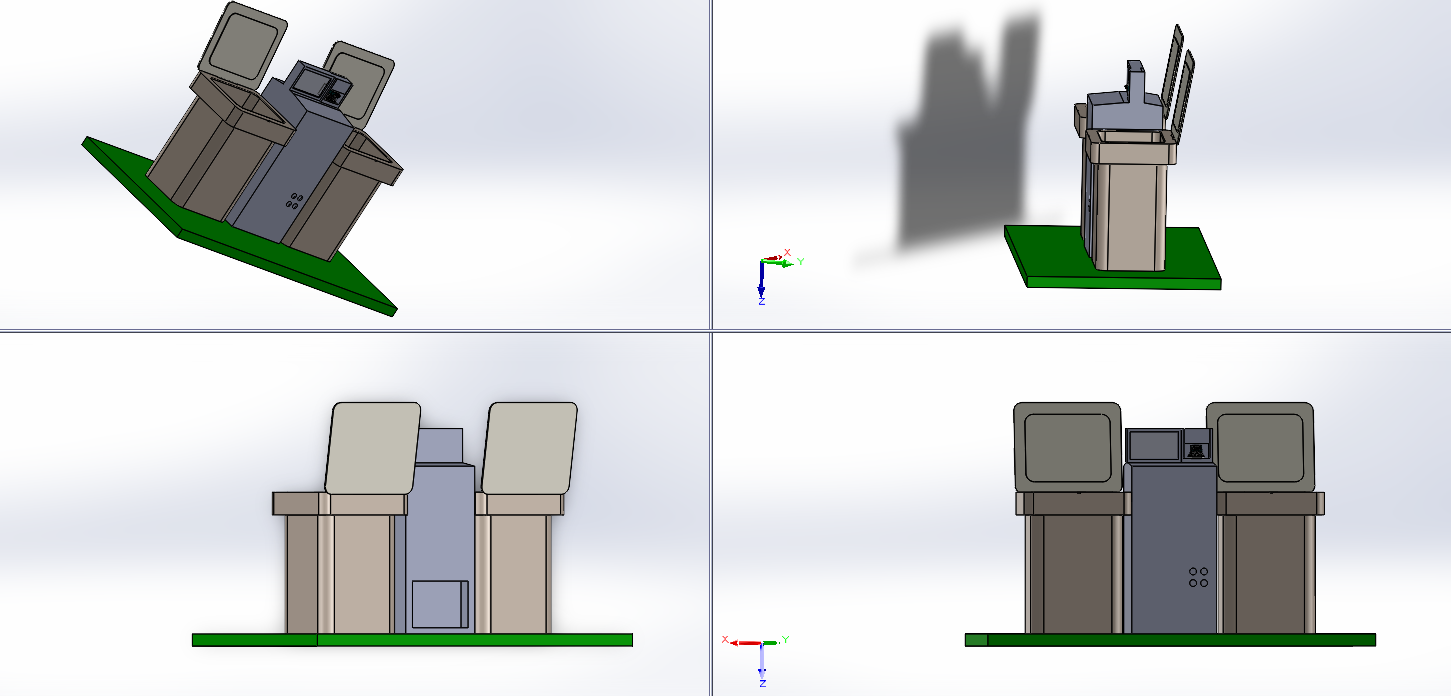
\includegraphics[width=6.89167in,height=3.50347in]{vertopal_24f0430788374a81b8d4c0bb6e5080ec/media/image5.png}

\emph{\textbf{Follow this link to view the detailed app design:}}

\url{https://www.figma.com/proto/SX6O9vvEQLcScNc1cOV6wi/Waste-Management-Apps-(Community)?node-id=1-60\&node-type=FRAME\&t=xxxKdC2mPkpmST5X-1\&scaling=min-zoom\&content-scaling=fixed\&page-id=0\%3A1\&starting-point-node-id=1\%3A60}

Click the link above to explore the app's features, user interface, and
interactive elements, designed to streamline waste management and reward
Eco-friendly behaviors!

\textbf{BUDGET}

\begin{longtable}[]{@{}
  >{\raggedright\arraybackslash}p{(\columnwidth - 6\tabcolsep) * \real{0.3259}}
  >{\raggedright\arraybackslash}p{(\columnwidth - 6\tabcolsep) * \real{0.1412}}
  >{\raggedright\arraybackslash}p{(\columnwidth - 6\tabcolsep) * \real{0.1988}}
  >{\raggedright\arraybackslash}p{(\columnwidth - 6\tabcolsep) * \real{0.3341}}@{}}
\toprule()
\begin{minipage}[b]{\linewidth}\raggedright
\textbf{Item Name}
\end{minipage} & \begin{minipage}[b]{\linewidth}\raggedright
\textbf{Quantity}
\end{minipage} & \begin{minipage}[b]{\linewidth}\raggedright
\textbf{Approximate Cost}
\end{minipage} & \begin{minipage}[b]{\linewidth}\raggedright
\textbf{Remarks}
\end{minipage} \\
\midrule()
\endhead
Sensor (for waste type detection) & 1 & ₹6,000 & Detects whether waste
is biodegradable or non-biodegradable \\
Motorized Lid Mechanism & 2 & ₹2,000 & For automatic bin opening based
on sensor input \\
Microcontroller (e.g., Arduino/Raspberry Pi) & 1 & ₹6,000 & To control
sensors and the motorized lids \\
Frame and Bin Stand & 1 & ₹1,500 & For supporting the two bins and
central sensor system \\
Dustbins (Biodegradable \& Non-biodegradable) & 2 & ₹4,500 & Separate
bins for different types of waste \\
Welding and Assembly Cost & 1 & ₹1,000 & For building and assembling the
structure \\
Power Supply Unit & 1 & ₹1,000 & To power the sensors, microcontroller,
and motors \\
Wires and Connectors & - & ₹500 & For connecting components and ensuring
stable power \\
Mobile App Development & 1 & ₹5,000 & For a different use case in the
project \\
Testing and Calibration Kit & 1 & ₹1,500 & To test and fine-tune the
sensor-based system \\
Miscellaneous (screws, mounts, etc.) & - & ₹1,000 & Additional small
parts needed for assembly \\
\textbf{TOTAL} & & \textbf{₹30,000} & \\
\bottomrule()
\end{longtable}

\hypertarget{bibliography}{%
\section{BIBLIOGRAPHY}\label{bibliography}}

\begin{enumerate}
\def\labelenumi{\arabic{enumi})}
\item
  \href{https://robu.in/}{https://robu.in}
\item
  \url{https://www.figma.com/community}
\item
\end{enumerate}

\end{document}
